\section{Hash}

\begin{frame}
	\begin{block}{Hash}
		\begin{itemize}
			\item São estruturas de dados feitas para garantir operações básicas como inserir, remover buscar em tempo constante independente do tamanho da estrutura.

			\item Para isso são assumidos alguns requisitos, como saber o tamanho total de elementos do conjunto e localizar uma função hash com espalhamento uniforme, em outras palavras poucas colisões.
			
			\item A primeira técnica de hash que estudaremos é o endereçamento direto. Usado quando o universo total de chaves é pequeno, não existem colisões entre duas chaves distintas e o tamanho da tabela de mapeamento direto é do tamanho do universo de chaves.

		\end{itemize}
	\end{block}
\end{frame}

\begin{frame}
	\begin{block}{Hash}
		\begin{itemize}
			\item Desenhar na lousa.

			\item Citar o exemplo de números: $D = {(1, "um"), (2, "dois"), \ldots (7, "sete"), (8, "oito") }$ .
				
			\item Citar o exemplo de palavras: Queremos construir um dicionário dinâmico simplificado, com $4$ palavras de no máximo $8$ letras. Este dicionário dinâmico pode ter somente as seguintes palavras: "concha", "casa", "hospital" e "time".

		\end{itemize}
	\end{block}
\end{frame}

\begin{frame}
	\begin{block}{Hash}
		\begin{itemize}
			\item No exemplo das palavras qual seria o tamanho do vetor de endereçamento?
	
			\item Vamos pensar... 
			
			\item Número de diferentes String’s de no máximo $8$ letras é:
			
			\item O que seria inviável em termos de memória! O número de palavras armazenados é bem menor do que esse conjunto total, ou seja, seria gasto muita memória alocando um vetor grande sem necessidade.
		\end{itemize}
	\end{block}
\end{frame}

\begin{frame}
	\begin{block}{Hash}
		\begin{itemize}
			\item Vamos supor que temos em média $500$ palavras, se o número de palavras do universo ultrapassar 500 teremos colisões.

			\item Todas as operações sobre a tabela hash devem ter complexidade assintótica constante $O(k)$ onde $k$ é constante.
			
			\item Colisões sempre vão existir, como podemos lidar com elas?
			
			\item Discutir com os alunos!
		\end{itemize}
	\end{block}
\end{frame}

\begin{frame}
	\begin{block}{Hash encadeamento}
		\begin{itemize}
			\item Supondo que cada célula do vetor seja um objeto em C\# que contenha uma chave, usada para indexar o hash e uma estrutura de dados lista ligada/árvore.

			\item Nesse caso sempre que ocorrer uma colisão teremos uma estrutura contendo os valores dentro.
		\end{itemize}
	\end{block}
\end{frame}

\begin{frame}
	\begin{block}{Hash encadeamento}
		\begin{itemize}
			\item Vamos supor uma função hash simples: $<<Key>> mod 7$, por exemplo. 
			
			\item Em seguida, adicionamos as chaves: $ 50, 700, 76, 85, 92, 73, 101$

		\end{itemize}
	\end{block}
\end{frame}

\begin{frame}
	\begin{block}{Endereçamento aberto}
		\begin{figure}[!htb]
			\centering	  				
			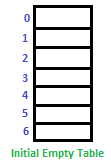
\includegraphics[height=3cm, width = 3cm]{./pic/hashChaining11.png}
			\caption{Endereçamento aberto  \cite{GEEKS_2018}}
		\end{figure}
	\end{block}
\end{frame}

\begin{frame}
	\begin{block}{Endereçamento aberto}
		\begin{figure}[!htb]
			\centering	  				
			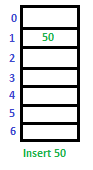
\includegraphics[height=3cm, width = 3cm]{./pic/hashChaining12.png}
			\caption{Endereçamento aberto  \cite{GEEKS_2018}}
		\end{figure}
	\end{block}
\end{frame}

\begin{frame}
	\begin{block}{Endereçamento aberto}
		\begin{figure}[!htb]
			\centering	  				
			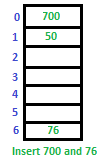
\includegraphics[height=3cm, width = 3cm]{./pic/hashChaining13.png}
			\caption{Endereçamento aberto  \cite{GEEKS_2018}}
		\end{figure}
	\end{block}
\end{frame}

\begin{frame}
	\begin{block}{Endereçamento aberto}
		\begin{figure}[!htb]
			\centering	  				
			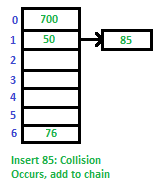
\includegraphics[height=3cm, width = 5cm]{./pic/hashChaining14.png}
			\caption{Endereçamento aberto  \cite{GEEKS_2018}}
		\end{figure}
	\end{block}
\end{frame}

\begin{frame}
	\begin{block}{Endereçamento aberto}
		\begin{figure}[!htb]
			\centering	  				
			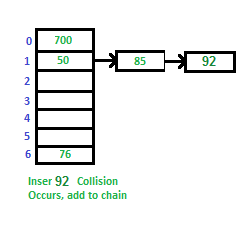
\includegraphics[height=3cm, width = 5cm]{./pic/hashChaining15.png}
			\caption{Endereçamento aberto  \cite{GEEKS_2018}}
		\end{figure}
	\end{block}
\end{frame}

\begin{frame}
	\begin{block}{Endereçamento aberto}
		\begin{figure}[!htb]
			\centering	  				
			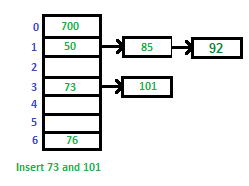
\includegraphics[height=3cm, width = 5cm]{./pic/hashChaining16.png}
			\caption{Endereçamento aberto  \cite{GEEKS_2018}}
		\end{figure}
	\end{block}
\end{frame}


\begin{frame}
	\begin{block}{Hash encadeamento}
		\begin{itemize}
			\item Quais seriam as vantagens e desvantagens dessa solução?
 
			\item Conversar com os alunos sobre isso.
		\end{itemize}
	\end{block}
\end{frame}

\begin{frame}
	\begin{block}{Hash encadeamento}
		\begin{itemize}
			\item Como vantagens temos:
			
			\item A simplicidade em implementar	
			
			\item A tabela não fica vazia pois podemos encadear mais nós com colisão nas listas ligadas	
			
			\item Usada frequentemente quando não temos certeza do número de elementos do conjunto
		\end{itemize}
	\end{block}
\end{frame}



\begin{frame}
	\begin{block}{Hash encadeamento}
		\begin{itemize}
			\item Como desvantagens temos:
			
			\item A performance do cache é inferior a abordagem de endereçamento aberto
				
			\item Desperdício de espaço, muitas células da tabela podem nunca ser usadas
				
			\item Se o encadeamento for longo, o tempo de  pesquisa tenderá a $O(n)$ o que não é bom
		
			\item Usa espaço extra para armazenar os links
		\end{itemize}
	\end{block}
\end{frame}


\begin{frame}
	\begin{block}{Hash endereçamento aberto}
		\begin{itemize}
			\item Com essa abordagem usamos apenas o vetor para armazenar todas as chaves. 

			\item Dessa forma, o tamanho da tabela tem que ser maior ou igual ao número de chaves totais do nosso universo. 
			
			\item Evidente que podemos copiar os dados antigos para uma nova tabela, no caso de estourar o tamanho máximo. Mas dentro do possível queremos evitar essa situação.
		\end{itemize}
	\end{block}
\end{frame}

\begin{frame}
	\begin{block}{Hash endereçamento aberto}
		\begin{itemize}
			\item Uma primeira solução é a sondagem linear, ao ocorrer uma colisão procuramos no slot seguinte se há espaço vazio. 

			\item No caso de ter espaço vazio, inserimos nele, caso contrário prosseguimos procurando mais slots vazios.
		\end{itemize}
		\begin{figure}[!htb]
			\centering	  				
			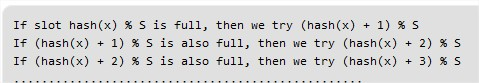
\includegraphics[height=2cm, width = 7cm]{./pic/sondagemLinearCode.jpg}
			\caption{Sondagem Linear  \cite{GEEKS_2018}}
		\end{figure}
				
		\begin{itemize}	
			\item A desvantagem desse método é que após a inserção de diversas colisões o tempo de pesquisa passa a ser linear.
		\end{itemize}
	\end{block}
\end{frame}

\begin{frame}
	\begin{block}{Hash: sondagem linear}
		\begin{itemize}
			\item Vamos supor uma função hash simples: $<<Key>> mod 7$, por exemplo. 
			
			\item Em seguida, adicionamos as chaves: $ 50, 700, 76, 85, 92, 73, 101$

		\end{itemize}
	\end{block}
\end{frame}

\begin{frame}
	\begin{block}{Endereçamento aberto}
		\begin{figure}[!htb]
			\centering	  				
			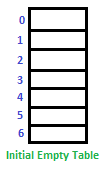
\includegraphics[height=3cm, width = 3cm]{./pic/openAddressing11Linear.png}
			\caption{Endereçamento aberto  \cite{GEEKS_2018}}
		\end{figure}
	\end{block}
\end{frame}

\begin{frame}
	\begin{block}{Endereçamento aberto}
		\begin{figure}[!htb]
			\centering	  				
			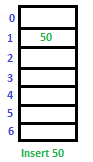
\includegraphics[height=3cm, width = 3cm]{./pic/openAddressing12Linear.png}
			\caption{Endereçamento aberto  \cite{GEEKS_2018}}
		\end{figure}
	\end{block}
\end{frame}

\begin{frame}
	\begin{block}{Endereçamento aberto}
		\begin{figure}[!htb]
			\centering	  				
			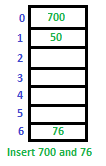
\includegraphics[height=3cm, width = 3cm]{./pic/openAddressing13Linear.png}
			\caption{Endereçamento aberto  \cite{GEEKS_2018}}
		\end{figure}
	\end{block}
\end{frame}

\begin{frame}
	\begin{block}{Endereçamento aberto}
		\begin{figure}[!htb]
			\centering	  				
			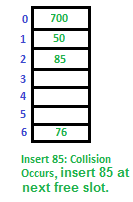
\includegraphics[height=3cm, width = 3cm]{./pic/openAddressing14Linear.png}
			\caption{Endereçamento aberto  \cite{GEEKS_2018}}
		\end{figure}
	\end{block}
\end{frame}

\begin{frame}
	\begin{block}{Endereçamento aberto}
		\begin{figure}[!htb]
			\centering	  				
			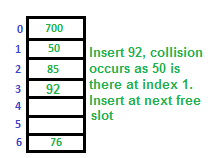
\includegraphics[height=3cm, width = 3cm]{./pic/openAddressing15Linear.png}
			\caption{Endereçamento aberto  \cite{GEEKS_2018}}
		\end{figure}
	\end{block}
\end{frame}

\begin{frame}
	\begin{block}{Endereçamento aberto}
		\begin{figure}[!htb]
			\centering	  				
			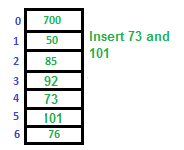
\includegraphics[height=3cm, width = 3cm]{./pic/openAddressing16Linear.png}
			\caption{Endereçamento aberto  \cite{GEEKS_2018}}
		\end{figure}
	\end{block}
\end{frame}

\begin{frame}
	\begin{block}{Hash: sondagem quadrática}
		\begin{itemize}
			\item Uma outra técnica usada é a sondagem quadrática. 

			\item Técnica que procura pela próxima posição vazia de célula elevada ao quadrado.
		\end{itemize}
				\begin{figure}[!htb]
			\centering	  				
			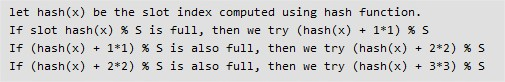
\includegraphics[height=2cm, width = 6cm]{./pic/quadratic.jpg}
			\caption{Endereçamento aberto quadrático  \cite{GEEKS_2018}}
		\end{figure}
	\end{block}
\end{frame}

\begin{frame}
	\begin{block}{Hash: sondagem quadrática}
		\begin{itemize}
			\item Exercício para os alunos aplicar o conceito de hash com sondagem quadrática para o exemplo anterior.
		\end{itemize}
	\end{block}
\end{frame}


\begin{frame}
	\begin{block}{Hash: hash duplo}
		\begin{itemize}
			\item Uma outra técnica usada é o hash duplo. 

			\item Técnica que usa duas funções de hash para encontrar o próximo slot vazio.
		\end{itemize}
				\begin{figure}[!htb]
			\centering	  				
			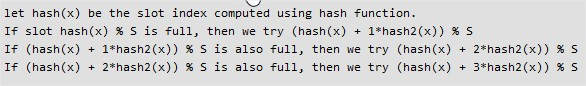
\includegraphics[height=2cm, width = 6cm]{./pic/doubleHash.jpg}
			\caption{Hash Duplo  \cite{GEEKS_2018}}
		\end{figure}
	\end{block}
\end{frame}


\begin{frame}
	\begin{block}{Hash: sondagem quadrática}
		\begin{itemize}
			\item Exercício para os alunos aplicarem o conceito de hash duplo para o exemplo anterior.
		\end{itemize}
	\end{block}
\end{frame}

\begin{frame}
	\begin{block}{Hash: sondagem quadrática}
		\begin{itemize}
			\item Usar a collection do C\# de hashtable:

			\item https://msdn.microsoft.com/pt-br/library/system.collections.hashtable(v=vs.110).aspx.
		\end{itemize}
	\end{block}
\end{frame}
 